%!TEX root = pfe-book4.tex
%!TEX TS-program = pdflatex
%!TEX encoding = UTF-8 Unicode


\cleardoublepage
%\mainmatter
\chapter[The Structure of Atomic Nuclei]{The Structure of \\Atomic Nuclei}
\label{ch-05}

\section{Isotopes}
In the third book of this series we told the story of how a flux of particles with different charge-to-mass ratios can be separated by means of electric and magnetic fields. And if the charges are the same, then separation of particles is possible as to mass. This is done by a device called a \emph{mass spectrograph}, which is widely used for chemical analysis.


A diagram of this instrument is shown in \figr{fig-5.1}. The underlying idea is as follows. Particles with different velocities enter the electric field of a capacitor. Imagine a group of particles with the same $e/m$ ratio. A flux of these particles enters an electric field and is separated into faster particles that exhibit a smaller deviation in the electric field and slower particles with a greater
deviation. In fan-like fashion, these particles then enter a magnetic field perpendicular to the drawing. It is con­nected so as to deflect the particles in the opposite di­rection. Here too, the faster particles are deflected less than the slower particles. From this it follows that at some point outside the field, the imagined flux of identical particles will again collect in a single point, that is to
say, they will come to a focus.

\begin{figure}[!ht]
\centering
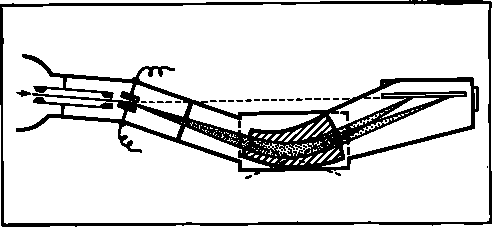
\includegraphics[width=0.9\textwidth]{figures/fig-05-01.pdf}
\caption{A schematic drawing of a mass spectrograph used for chemical analysis.}
\label{fig-5.1}
\end{figure}


Particles with a different $e/m$ value will also collect in a point, but that will be a different point. Calculations show that the foci for all $e/m$ values will lie very close to a certain straight line. Now if a photographic plate is positioned along this straight line, particles of each kind will reveal themselves by a separate line.

Isotopes were discovered with the help of a mass spec­trograph. The honour for the discovery of isotopes goes to Sir Joseph John Thomson. In 1913, while studying the deflection of a beam of neon ions in an electric field and a magnetic field, he noticed that the beam was sepa­rated into two parts. The atomic weight of neon was known with sufficient accuracy: \num{20.200}. It was found that in reality there are three kinds of neon atoms, with atomic weights 20, 21, and 22. Sorry, I’m rather used to the old terms; these numbers are now called relative atomic masses.

Since the chemical properties of neon do not depend on their masses, physicists were soon confident that the differences are connected only with the nucleus. The charge of the nucleus and the number of electrons are the same and so different kinds of atoms of neon should occupy the same place in Mendeleev’s periodic table of elements. Whence the name, \emph{isotopes}, or those that occu­py the same place.

In the 1920s, the mass spectrograph took on its present-day features and a study began of the isotopic compo­sition of all elements. All elements, without exception, constitute a mixture of isotopes. There are some, like hydrogen and oxygen, that consist mainly of one isotope (hydrogen of mass 1--99.986\%, oxygen of mass 16--99.76\%). There are others that contain different isotopes in about equal quantities. Say, chlorine (75\% is an isotope of mass 35 and 25\% is an isotope of mass 37). There are still other elements that consist of a large num­ber of isotopes. The examples we have given are those of stable isotopes. Radioactive isotopes of an element (these are not stable and decay) will be discussed later on.

The mass spectrograph was soon refined to the point where it was established that the masses of isotopes are expressed by whole numbers only up to the second to fourth decimal place. The reasons for this deviation will be taken up later on.

The mass of an atom rounded off to a whole number is called the \emph{mass number}.

Since the nuclear mass does not affect the chemical behaviour of an element, there are obviously many chem­ical compounds that differ in their isotopic composition. For example, there are two kinds of water, ordinary water and heavy water. In ordinary water, we find an isotope of hydrogen with mass number 1, in heavy water (called deuterium), the isotope of hydrogen has mass number 2. In the natural state, we find three isotopes of oxygen (mass numbers 16, 17, and 18), which means that water is a mixture of molecules of six different kinds. If the molecules of a substance consist of a large number of different atoms, then the number of isotopic varieties may run into the tens and hundreds.

Separating isotopes is an important branch of industry. And it is particularly important in a number of processes involved in the generation of atomic energy. Heavy water has to be separated from ordinary (light) water, different types of atoms of the nuclear fuel (uranium and thorium) have to be separated as well. And there are many many more such industrial problems that confront the physicist.

The complexity of the problem is that the atoms exhib­it extremely small differences in their electronic makeup and, hence, in their chemical properties. In the case of light atoms, the separation procedure is carried out with extreme difficulty in the form of a multistage chemical extraction process. In the case of heavy atoms, the only possible way is to apply physical methods that make use of slight differences in the masses of atomic nuclei.

The most widely employed method today is the gaseous diffusion method. Molecules containing isotopes of different mass differ slightly as to their rates of passage through a porous barrier. Light-weight molecules get through faster than the heavier varieties.

Of course, the separation procedure could be based on the principle of the mass spectrograph that we have just discussed. But both methods are time- and money-consuming.

Only just two or three years ago it was demonstrated that isotope separation can be handled by a new laser method. The most important advantage here is that the laser generates a ray of extremely high monochromicity. Now the difference in distances between energy levels occupied by electrons in two isotopic varieties of the same element is naturally very slight. This is due to the mass difference of the nuclei since the charges on the nuclei of two isotopes are the same. And it is precisely the charges that determine, on the whole, the location of the electronic levels. Now a laser beam is so strictly monochromatic that it is capable of exciting only one kind of isotope while leaving atoms of the other variety unexcited.


\begin{figure}[!ht]
\centering
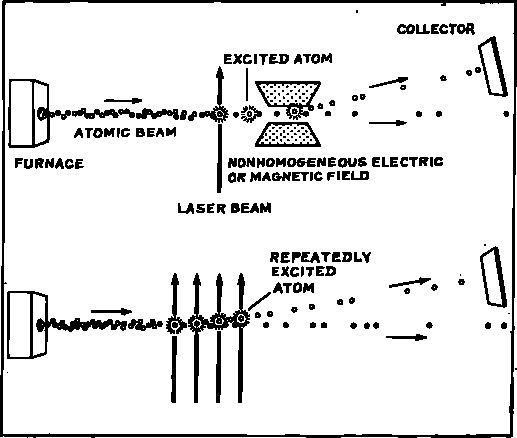
\includegraphics[width=0.9\textwidth]{figures/fig-05-02.pdf}
\caption{The separation of isotopes by means of a laser.}
\label{fig-5.2}
\end{figure}


\figr{fig-5.2} depicts two processes for separating isotopes by means of a laser. A gas made up of atoms or molecules emerge from an opening in a furnace. The laser beam excites the atoms of one isotopic variety. As a rule, the excited atoms possess an electric or magnetic moment, and so a nonhomogeneous magnetic or electric field will deflect them to one side (upper diagram).

A second method is used if the excited atoms are rapidly de-excited. In this case, the same atom passes through the space covered by a laser beam and is excited a second time, thus several times experiencing inelastic collisions with photons. Each absorption of a photon imparts to the atom a momentum that is in the direction of the action of the laser beam. Atoms that can be excited are simply pushed upwards whereas atoms of the variety that does not absorb photons are not deflected in their motion.


The first successful experiment of this kind was carried out with a beam of barium atoms irradiated with a laser beam of wavelength \num{0.55535} micrometre. Absorption of a single photon shifted the atom through \SI{0.8}{\centi\meter\per\second} in the case of a longitudinal velocity of \SI{50 000}{\centi\meter\per\second}.

\section{Radioactivity}
In the third book of this series a short description was given of how Rutherford established that the atom consists of a minute nucleus and of electrons moving around the nucleus. Now comes one of the most important chapters in physics. It describes the structure of the atomic nucleus, which is made up of protons and neutrons. Strange as it may seem, the history of this discovery began fifteen years before Rutherford demonstrated his nuclear model of the atom in experiments devoted to the scattering of alpha particles by a thin piece of foil.

In the spring of 1896, the French physicist Antoine Henri Becquerel (1852-1908) found that uranium emits rays that act much like $X$-rays. Just like the $X$-rays of Roentgen discovered several months before, the uranium rays fog photographic plates and pass through opaque objects. Their absorption is proportional to the density of the object placed between the uranium and a photo­ graphic plate. If the body is opaque to these rays, the outlines of the object are formed on the plate. The urani­um rays, like $X$-rays, are capable of ionizing air; the amount of ionization of the air is a good measure of their intensity.

What is similar in the discoveries of Becquerel and Roentgen is the element of chance: they were accidental.

But an accident all by itself is never the source of an im­portant scientific discovery. Just as there were people who had ``seen'' $X$-rays several years before Roentgen, so there were (as it turned out following Becquerel’s discov­ery) at least three people who had noticed the blackening of a photographic plate that had happened to be near uranium salts. But to ``see'' is one thing, and to pay attention to and locate the actual cause of the phenome­non is quite another thing. That is precisely what Roent­gen and Becquerel did and what their predecessors failed to do. Hence the honour and the glory go to them.

The path to Becquerel’s discovery went through the following stages. In the first tubes, the $X$-rays fell on glass. The glass fluoresced under the action of cathode rays. And so it was natural to think that the penetrating rays accompanied fluorescence. Becquerel began by con­ducting experiments with substances that exhibit fluo­rescence under the action of the sun’s rays. He was rather quick to see that the penetrating rays emanated from a variety of minerals containing uranium. That was a discovery. But Becquerel was in no hurry to report what he had found to the scientific community. The experi­ments were repeated a number of times. And it happened that the sun, out of spite, refused to come out of the clouds for several days. The photographic plates together with the mineral specimens lay in a drawer of his laboratory desk for a few days. On March 1, 1896, the sun finally came out and he could resume his experiments. But before doing so, Becquerel decided to check the qual­ity of his plates. He went into the dark room, developed one of the plates and saw the clear-cut outlines of his mineral specimens. Now there had not been any fluorescence and so that could not have been the cause.

Becquerel repeated the ``dark'' experiments and was convinced that his minerals were the source of the penetrating radiation that develops all by itself, without any help from light outside.


%\newpage
\begin{center}
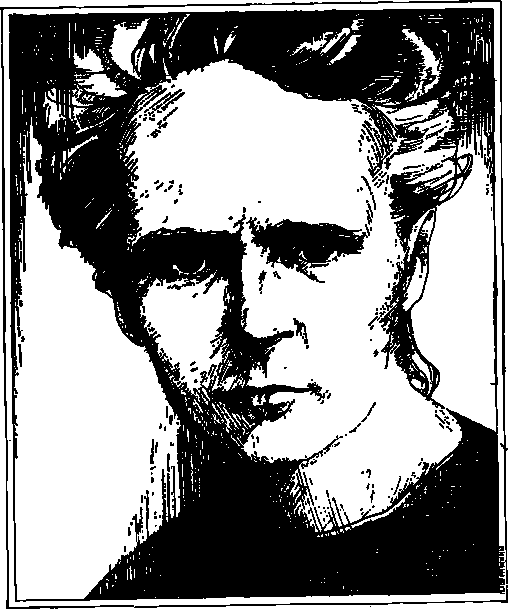
\includegraphics[width=0.8\textwidth,angle=-0.5]{figures/curie.pdf}
\end{center}
%\vspace{-.5cm}
{\small \textsf{{Marie Sklodowska Curie [1867-1934]}} -- \textsf{\footnotesize outstanding woman scien­tist. In 1898, while studying the emission of uranium and thorium (the nature of the emission was not known at that time), she discovered in the ores of these elements certain substances that pos­sess a far greater emission capability. She then isolated polonium and radium. Marie Curie and her husband Pierre Curie (1859-1906) introduced the term ``radioactive''. The discoveries of Marie Curie were immediately taken up by Rutherford and led to the laws of the radioactive decay of atoms.}}


A careful examination of many samples suggested to Becquerel that the source of the rays is uranium. If a mineral did not contain uranium, there was no penetrat­ing radiation. And to complete the proof he decided to make a study of pure uranium. But uranium is a rare element. Becquerel asked his friend, the French chemist Henri Moissan (1852-1907), for some. At a meeting of the French Academy of Sciences, Moissan told of a method for obtaining pure uranium, and Becquerel reported that uranium emits rays. These papers were delivered on No­vember 23, 1896. Only fifty years separate that discovery from the atomic bomb that was dropped on Hiroshima.

A year passed and in the autumn of 1897, two young physicists, the Curies -- a man and wife team -- began their experiments in a cold shed. But they worked with enthu­siasm. Marie Sklodowska Curie (1867-1934) chose for the topic of her dissertation a study of the chemical pecu­liarities of mineral specimens that generate the penetrat­ing radiation of Becquerel.

The intense work led from one discovery to another. First of all, it was found that, in addition to uranium, thorium also exhibits these penetrating rays. The inten­sity of the emission was measured by the intensity of the ionization current. Curie substantiated Becquerel’s con­jecture that the intensity of the penetrating rays does not depend on the composition of the chemical compounds involving uranium and thorium, and is strictly propor­tional to the number of their atoms.

Then came a setback: the uranium pitchblende ore yields four times more ionization than it should if it contained uranium. It is just at moments like these that the talent of the investigator is so important. An ordinary person would assume that the atoms of uranium were to blame. But Marie Curie realized that this phenomenon could be explained in a different way. It might be that the pitchblende ore contains a small quantity of some hitherto unknown chemical element capable of extremely powerful penetrating radiation.

The conjecture turned out to be true. The titanic work that Marie Curie carried out revealed a new element called \emph{polonium} (in honour of Marie’s home country Poland) and then \emph{radium} (meaning ray). Radium turned out to be nearly a thousand times more active than pure uranium.

Now let us go more quickly, paying less attention to the historical sequence of events.

Following the discovery of radium, other substances were found that were sources of penetrating radiation. They all received the name ``radioactive''.

What is this radioactive radiation?

A radioactive specimen was placed in an evacuated box and this was surrounded by a lead shield with a slit. The rays passed through the slit, fell on a photographic plate, and left a trace on it. But as soon as the box was placed between the poles of a magnet, the devel­oped plate revealed three marks. The radioactive beam had split up into three rays. One ray was deflected as if it were a flux of negatively charged particles, a second ray constituted a flux of positively charged particles, and one ray was not deflected at all. It was apparently somehow related to the $X$-rays.

By methods we have already discussed it was demon­strated that, in the general case, radioactive radiation consists of a flux of electrons (before it was known that they are electrons they were called \emph{beta rays}), a flux of atomic nuclei of helium (called \emph{alpha particles}), and some kind of hard electromagnetic radiation (called \emph{gam­ma rays}).

\section{Radioactive Decay}
Does something happen to the atoms that are sources of radioactive radiation? Yes, indeed. And these events are quite amazing. In 1902, our old acquaintance Sir Ernest Rutherford (1871--1937) (we have already told -- disregard­ing the historical sequence of events -- about his discovery of the structure of the atom in 1911) demonstrated that as a result of radioactive radiation there occurs a transfor­mation of one kind of atom into another kind.

Rutherford expected that this supposition, though based on rigorous experimental proof, would be challenged vigorously by chemists. True enough. The point is that by proving the transformation of atoms, we encroach on the holy of holies -- the indivisibility of the atom. By asserting that we can obtain lead from uranium we are accomplishing the dream of alchemists, who have merited as much ``glory'' as astrologists.

But under the weight of proof, the critics quickly retreated, and after some time the phenomenon of natural radioactive decay of certain atoms was incontestably demonstrated both by chemical and physical methods. What is the essence of radioactive transformation?

To begin with, it turned out that the electron rays that make up part of the radioactive radiation emanate from the nucleus. But if that is so, the charge on the nucleus increases by unity and the radioactive atom is converted into an atom next in order in the periodic table of elements.

An alpha particle carries a double positive charge and has a mass four times that of the hydrogen atom. If a nucleus ejects such particles, the atom must be ``dis­placed'' to the left in the periodic table of elements with an accompanying isotopic transformation.

It is almost too trivial to say that unstable atoms are subject to radioactive disintegration.

We do not know whether there were many such types of atoms when the earth began to cool off. But we have an excellent idea of what types of unstable atoms can now be found in nature. It turns out that they are members of three families, the progenitors of which are the uranium atom of mass number 238, the uranium atom of mass number 235, and the thorium atom of mass number 232.

\begin{figure}[!ht]
\centering
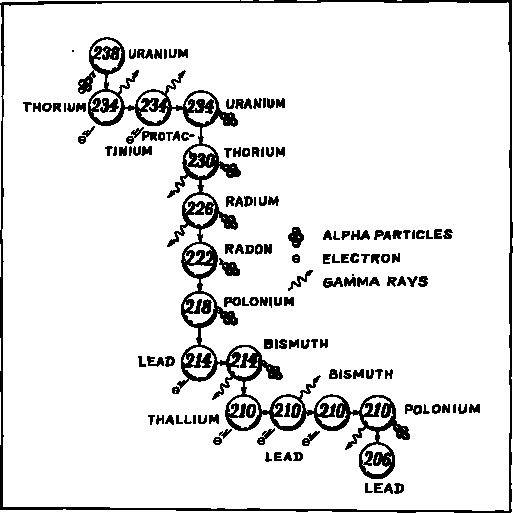
\includegraphics[width=0.9\textwidth]{figures/fig-05-03.pdf}
\caption{The decay modes of Uranium 238.}
\label{fig-5.3}
\end{figure}


\figr{fig-5.3} depicts the first family. The first transfor­mation is the transition of \ce{^{238}U} to \ce{^{234}Th}; this occurs due to the ejection of alpha particles. This is followed by two beta transformations that carry thorium to prot­actinium and then protactinium to uranium, but this time it is a uranium isotope of mass number 234. Then follow five consecutive alpha transformations that carry us down to the unstable isotope of lead of mass number 214. Another two zigzags and the process of disintegration comes to a halt: the lead isotope of mass number 206 is stable.

The destruction of each single atom is a random event. There are atoms that are ``lucky'' and have a long life­ time, others live for a fleeting moment.

But it is impossible to guess in any specific case when the given atom will be converted. We cannot name the date of demise of our cat or dog, but every animal species has its mean life span. And the same goes for every kind of atom: each has a very strict mean time of existence. Of course, atomic behaviour differs fundamentally from animal life. The life of unstable atoms, in contrast to the mean life span of living beings, does not depend on any external conditions. Nothing at all can affect what is called the mean decay time. Always, the same portion of atoms decays in unit time:
\begin{equation*}%
\frac{\Delta N}{N} = \lambda t
\end{equation*}
This formula holds true only for the case where the frac­tion ${\Delta N}/{N}$ is small.

The quantity $\lambda$ is a constant for every radioactive transition. Instead of employing that constant, it is more pictorial to characterize the rate of the process by the ``half-life'', which is the time during which half of any given quantity of radioactive material is transformed. For different radioactive elements, this time can have an enormous range. For example, the half--life of the progenitor of the \ce{^{238}U} family is equal to 4.5 thousand million years. Contrast that with the fact that half of the atoms of the lead isotope of mass number 214 decays in one millionth of a second.



%\newpage
\begin{center}
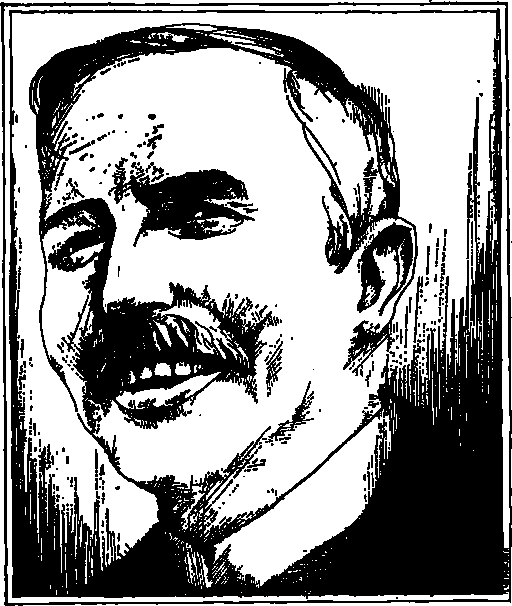
\includegraphics[width=0.8\textwidth]{figures/rutherford.pdf}
\end{center}
%\vspace{-.5cm}
{\small \textsf{{Ernest Rutherford [1871--1937]}} -- \textsf{\footnotesize the eminent British physicist and a great experimenter. In delicate and highly original experi­ments he demonstrated the essence of radioactive decay. In his classical experiments in the scattering of a flux of alpha particles by a substance, he substantiated the modern theory of the structure of the atom as a system consisting of a nucleus and electrons moving about the nucleus. Continuing his experiments involving the bom­bardment of different targets with nuclei, he was the first to achieve an artificial transmutation of elements.}}




\section[Nuclear Reactions]{Nuclear Reactions and \\the Discovery of the Neutron}

Radioactive transformations are quite similar to the chemical reaction of disintegration. Take a chemical sub­ stance, subject it to heat or light, and we obtain two substances. Say, carbonic acid breaks up into water and carbon dioxide, which is like what we have just consid­ered: a thorium nucleus of mass number 230 decays into a radium nucleus and a helium nucleus.

If nuclear disintegration is possible, then there must be nuclear reactions that take place via the principle
\begin{equation*}%
A+B \to C+D
\end{equation*}
To obtain a chemical reaction of this kind, we have to mix the molecules of substances $A$ and $B$. To achieve a nuclear reaction, we have to bring into collision two atomic nuclei.

Those were the experiments that Ernest Rutherford (1871-1937) began in 1919. This was before the time of particle accelerators, and nuclear reactions were achieved by means of bombarding a substance with alpha parti­cles. After powerful fluxes of protons and other nuclei were obtained, new nuclear reactions were discovered. It became clear that in principle an isotope of any chemi­cal element could be converted into another isotope. Even gold could be obtained from other substances. The dream of alchemists had become reality. The first nuclear reaction discovered was of the type $A+B \to C+D$, it was the conversion of nitrogen and helium into oxygen and hydrogen. We can write down this reaction as follows:
\begin{equation*}%
\ce{{^{14}_{7}N} + {^{4}_{2}He} -> {^{17}_{8}O} + {^{1}_{1}H}}
\end{equation*}
Note that the sums of the superscripts and the sums of the subscripts remain unchanged. The subscripts indicate the charge on the nucleus, the superscripts the mass rounded off to a whole number, that is, the mass numbers. Thus, the law of conservation of electric charge is main­tained rigorously. As we shall see later on, the law of conservation of mass is only approximate. And, finally, the sum of the mass numbers is preserved just as strictly as the charge.

As early as 1920, Rutherford suspected that there must be a particle devoid of electric charge and close to the proton in mass. Otherwise, he said, it is difficult to understand how a positively charged alpha particle can penetrate into a positively charged nucleus, since like charged particles repel.

The particle without a charge -- the \emph{neutron} -- was dis­covered in 1932. It is easy to see why its discovery was ``held up'' The point is we see charged particles through the tracks they leave in a gas or a photographic emulsion due to ionization of the molecules they encounter in their path. But an electrically neutral particle does not interact with electrons and therefore it does not leave any tracks. We can judge the existence of neutrons only on the basis of secondary effects.

The neutron was discovered in the bombardment of beryllium with alpha particles. This reaction can be writ­ten down thus:
\begin{equation*}%
\ce{{^{9}_{4}Be} + {^{4}_{2}\alpha} -> {^{12}_{6}C} + {^{1}_{0}n}}
\end{equation*}
The symbol $n$ stands for neutron. But how can we be sure of the existence of a particle that does not itself leave any traces? On the basis of its actions. Imagine an invisible billiard ball on a billiard table. A visible ball is rolling over the green cloth and suddenly, inexplica­bly, bounds off to the side. The physicist cannot sus­pect the laws of conservation of energy and momentum to have gone wrong. And so he concludes that the visible ball collided with an invisible ball. What is more, by applying the conservation laws he is able to determine all the characteristics of the invisible ball; this he does by computing the angle of deviation from the line of flight and the change in velocity of the visible ball.

The number of neutrons is calculated in the following way. A substance containing boron atoms is placed in the path of a neutron beam. When a neutron encounters a boron nucleus it ceases to exist. The reaction that occurs is the following:
\begin{equation*}%
\ce{{^{10}_{5}B} + {^{1}_{0}n} -> {^{7}_{3}Li} + {^{4}_{2}\alpha}}
\end{equation*}
The neutron vanished but an alpha particle came into being. By recording these charged particles that leave visible tracks in a variety of devices, we can make exact measurements of the intensity of a neutron beam.

There are many other methods for determining, with complete assurance, all the parameters that characterize a neutron and, generally, any electrically neutral particle. An assemblage of precisely matched indirect findings is sometimes no less convincing than actually seeing visible traces.

\section{Properties of Atomic Nuclei}

Prior to the discovery of the neutron, physicists pic­tured the atomic nucleus as consisting of electrons and protons. This involved many contradictions, and at­tempts to create a theory of nuclear structure were all failures. As soon as the neutron was found in nuclear collisions, the idea immediately arose that the atomic nucleus consists of neutrons and protons. This hypothesis was first advanced by the Soviet physicist D. D. Iva­nenko.

It was clear from the very start that the neutron mass was very close, if not equal, to the proton mass. This immediately gave rise to a clear--cut interpretation of the differences between isotopes of one and the same element.

As we see, to each isotope we can ascribe two numbers. One is the ordinal number in the periodic table of ele­ments, $Z$, which is equal to the number of protons in the nucleus. The ordinal (or atomic) number determines the number of electrons associated with the nucleus. Now if that is so, then it is clear that the atomic number must be responsible for the chemical behaviour of the elements (this is because chemical reactions do not involve nuclei).

Now the mass number is equal to the total number of neutrons and protons, and so isotopes of one and the same element differ as to the number of neutrons in the nucleus.

Very precise experiments have elicited the character­istics of both particles that make up atomic nuclei. The mass of the proton is equal to \SI{1.6726d-24}{\gram}, which is 1836 times more massive than the electron. The proton has a spin of 1/2 and a magnetic moment equal to \num{1.41d-23} unit in the centimetre-gram-second system. The mass of the neutron is slightly greater than the mass of the proton, namely, \SI{1.6749d-24}{\gram}. The neutron has spin 1/2. The magnetic moment of the neutron is antipar­allel to the spin and is equal to \num{0.966d-23} unit in the centimetre-gram-second system.

The spins and magnetic moments of atomic nuclei are studied by a variety of methods: use is made of optical spectroscopy, radiospectroscopy, studies of the deflection of beams of particles in a nonhomogeneous magnetic field. The general principles of these methods were discussed in the third book of this series and in the preceding chapters of this book. Here we will confine ourselves merely to a presentation of the basic facts obtained in the past few decades by large band of physicists.

First of all, I would like to stress that the laws of quantum physics pertaining to the moment of momentum (or angular momentum) hold true for all particles. And so for atomic nuclei we can write the formula for the angular momentum as:
\begin{equation*}%
\sqrt{S(S+ 1)}\,\frac{h}{2 \pi}
\end{equation*}
Here, the quantity $h$ is the Planck constant that we encounter in all formulas of quantum physics.

Usually the spin is the parameter $S$ and not this ex­pression. Theory states rigorously and experiment demon­strates brilliantly that the spin of every particle has to be equal to 0, 1/2, 1, 3/2, and so forth.

Looking through the tables of values of spin of different atomic nuclei (obtained in a variety of experiments), we find a number of interesting regularities. First of all, in nuclei with an even number of protons and an even number of neutrons, the spin of the nucleus is equal to zero (\ce{He}, \ce{^{12}C}, \ce{^{16}O}). The number of nucleons (that is, nuclear particles) that is a multiple of four apparently plays a very big role. In many cases (though not in all) the spin of the atomic nucleus may be obtained as follows: drop the number closest to the mass number $A$ that is a multiple of four and multiply the difference by 1/2. For example: in lithium--6 the spin is $2 \times 1/2 = 1$; it is 3/2 in lithium--7, 1 in boron--10, and 3/2 in boron--11.

The rule is rather obvious: nuclei with an even mass number $A$ have integral spin or spin zero, nuclei with odd $A$ have spin equal to a multiple of 1/2.

The \emph{Pauli exclusion principle} is applicable to both protons and neutrons in the nucleus. Two identical parti­cles can reside in one energy level only if the spins are antiparallel. Since the proton and the neutron are different particles, one level can accommodate two protons and two neutrons. In this compact group with spin zero we perceive the helium atom (the alpha particle).

The presence of spin means the presence of a magnetic moment. As we know, there is a relationship of direct proportionality between the mechanical momentum $L$ and the magnetic moment $M$. Here, the magnetic moment may be either parallel or antiparallel to the spin.

\section{Bosons and Fermions}
We have emphasized time and again that one energy level can accommodate only two particles with opposite spins. The time has come to say that this principle (the Pauli exclusion principle) holds true only for one class of particles. They are called \emph{fermions}. The fermions in­clude electrons, protons, and neutrons, and also all other particles that consist of an odd number of fermions. There is a second class of particles called \emph{bosons}. The bosons include the photon, a number of short-lived elementary particles (like, say, the pi-meson) and (most im­portant of all) all particles that consist of an even number of fermions.

\begin{figure}[!ht]
\centering
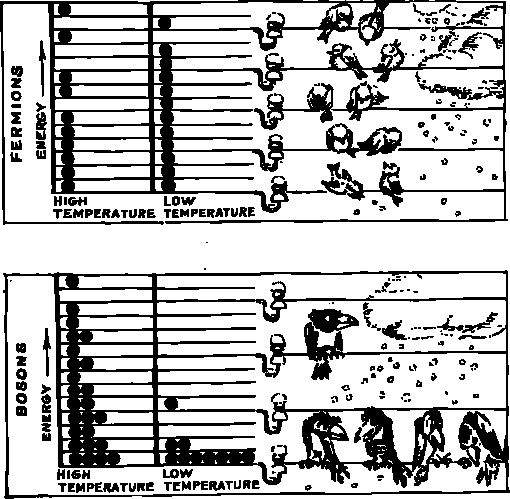
\includegraphics[width=0.9\textwidth]{figures/fig-05-04.pdf}
\caption{The difference in bosons and fermions while occupying energy levels.}
\label{fig-5.4}
\end{figure}

There is no limit to the number of bosons that can occupy one energy level. To get a better grasp of the difference between bosons and fermions, take a look at \figr{fig-5.4}. Here, each black dot symbolizes a pair of particles with opposite spins. At very low temperatures, bosons mainly congregate on the lowest possible energy level. In this drawing, fermions appear as a column.

It is quite obvious that the differences in the behaviour of fermions and bosons are most obvious at low tempera­tures. At the very lowest temperatures, the number of bosons located in the ``cellar'' may be almost equal to the total number of bosons.
Don’t try to ``understand'' what we have just said. Just remember it, because what we have said is really the ultimate truth. But I am very sorry every time I have to tell the reader (without offering proof) about things that can only be demonstrated with the aid of very in­volved mathematical equations. It turns out that in cer­tain cases bosons can, in other cases cannot, congregate on a single energy level in large numbers. If they can, we say a \emph{Bose--Einstein condensation} has taken place.

When a large number of particles congregate on one level, their motion becomes ideally matched. Twin par­ticles move about identically despite the thermal chaos.
In the second book of this series we spoke of a marvel­ous liquid that possesses superfluidity at low tempera­tures. This liquid is a collection of \ce{^{4}He} (helium) atoms.

The atoms of this isotope are bosons. At a temperature of 2.19 degrees above absolute zero there occurs a conden­sation of the particles that imparts to the liquid an amazing property: superfluidity. The loss, of friction may be explained in very rough fashion as follows: if only one atom gets through an extremely narrow slit, all the others follow suit immediately.

Actually we are dealing with two phenomena, where a flux of particles moves without regard for obstacles. The superfluid flow of \ce{^{4}He} atoms resembles electric current with zero resistance which is found in many metals and alloys and also at low temperatures.

But electrons are fermions. They cannot congregate together. The way out of this impasse was found in 1956 when three American scientists proposed a theory in accordance with which electrons can form into pairs below a certain temperature; and as we pointed out at the very start, a pair of fermions is a boson. Consequently, super­ conductivity sets in when such bosons condense on a single energy level. These two remarkable phenomena, \emph{superconductivity} and \emph{superfluidity}, have one and the same explanation. A single particle picks out a path that is ``more suitable'' and all other particles follow it.

If the idea of the conversion of fermions into bosons due to coupling into pairs is true, then we may ask: Can the isotope of helium of mass number 3, which has spin and is a fermion, become superfluid like \ce{^{4}He}?

It was evident from the very beginning that if this phenomenon does exist, then at any rate at temperatures much lower than the temperature of the transition of the basic isotope of helium, \ce{^{4}He}, into the superfluid state. The reason is clear: the nucleus of the \ce{^{3}He} atom consists of two protons and one neutron, which means it is 25\% lighter than its brother. Therefore, naturally, its thermal motion will be more intense and setting up a march of bosons will become possible at lower temperatures. But at what temperatures? Unfortunately, theory could not predict the transition temperature of \ce{^{3}He} to the superfluid state. Fantastic persistence and the overcoming of enormous difficulties were needed before superfluid (\ce{^{3}He}) helium was obtained in 1974.

And at what temperature does the transition occur? It would be most appropriate to print the answer in bold­ face type: \textbf{at 0.0027 degree Kelvin}. And if the reader thinks that the two--degree difference between that and ordinary \ce{^{4}He} helium is nothing much to speak of, he has another thought coming. This is not at all like the difference between \SI{20}{\celsius} and \SI{18}{\celsius}. In this everyday event, the temperature fell by a factor of 293/291, whereas in the case we are discussing it dropped 1000 times -- a tremendous achievement of experimental physics and a triumph of theoretical physics that predicted the coupling of atoms of \ce{^{3}He} into a ``boson'' pair.

\begin{figure}[!ht]
\centering
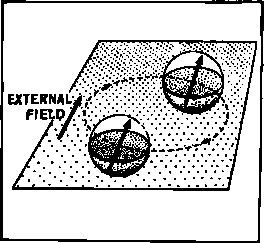
\includegraphics[width=0.5\textwidth]{figures/fig-05-05.pdf}
\caption{The coupling of magnetic moments of two atoms.}
\label{fig-5.5}
\end{figure}

A visual image might help in understanding and re­membering this. Take a look at \figr{fig-5.5}. The magnetic moments of two atoms are in the same direction. Thus, the transition of \ce{^{3}He} into a state of Bose--Einstein con­densation must be accompanied by a jump-like change in the frequency of the magnetic resonance. The point is that the pair behaves like a single whole, which is precisely what was detected in the experiment. This was such a brilliant page in the history of physics that it would have been a pity not to have told the reader about it despite any possibility of explaining under what con­ditions and on the basis of what events fermions couple up into boson pairs.

\section[The Mass and Energy of an Atomic Nucleus]{The Mass and Energy \\of an Atomic Nucleus}
It was mentioned in passing that the mass number rounds the exact value of the mass of the nucleus to a whole number.

The accepted way today (this was discussed in the first book) is to choose the atomic mass unit as 1/12 of the mass of the carbon isotope \ce{^{12}C}.

The relative masses of the isotopes of all atoms differ from whole numbers very slightly but still so substan­tially that we cannot attribute these differences to exper­imental errors. The mass of is equal to 1.00807, the mass of deuterium is not at all twice as much, it is equal to 2.01463.

A careful study of the tables of isotopic masses shows that the mass of the nuclei is less than the sum of the masses of the elementary particles that constitute the new nucleus. For example, the mass of a neutron is 1.00888, the proton mass is 1.008807; the mass of two neutrons and two protons is equal to 4.0339, yet the mass of the nucleus of a helium atom, which consists of two neutrons and two protons, is not equal to that number, but to 4.0038. Thus the mass of the helium nucleus is less than the sum of the masses of the component parti­cles of the nucleus by the amount of 0.0301 atomic unit, which is thousands of times greater than the measurement accuracy.

There can be no doubt that these small differences have a profound meaning. What is it?

The answer is given by the theory of relativity. Its appearance on the stage at that moment was undoubtedly more effective than when experiment confirmed the de­pendence of the electron mass on the velocity of the elec­tron. The fact that the sum of the masses of the protons and neutrons making up the nucleus is less than the mass of the nucleus (this is termed the \emph{mass defect}) is interpreted precisely and clearly with the aid of the famous equation $E =mc^{2}$. If a system acquires or loses an amount of energy $\Delta E$, then the mass of that system increases (or, respectively, decreases) by the quantity
\begin{equation*}%
\Delta m = \frac{\Delta E}{c^{2}}
\end{equation*}
The mass defect of the nucleus (from the viewpoint of this principle) thus receives a very natural interpreta­tion: it is the measure of the binding energy of the nuclear particles.

In chemistry and physics, the \emph{binding energy} is under­ stood to be the work which has to be expended in order to disrupt the given bond completely. If it were possible to split the nucleus up into elementary particles, then the mass of the system would increase by the amount of the mass defect $\Delta m$.

A breaking up of the nucleus would lead to the release of a tremendous amount of energy. It is simple to calcu­late that a change in mass by one thousandth of a relative unit, that is, by \SI{1.66d-27}{\gram}, is equivalent to approx­imately 1 million electron volts.

Knowing the atomic mass of the nucleus, the reader will immediately see something very interesting. If we divide the energy binding the protons and neutrons in the nucleus by the number of particles, we get one and the same number, namely, \SI{8}{\mega\electronvolt} (megaelectron volts, or million electron volts) for all nuclei, with the exception of some of the very lightest ones. From this there most definitely follows an important consequence: only the closest lying protons and neutrons interact, which means nuclear forces operate over short distances and become practically zero if one recedes from the proton or neutron to distances of the order of the dimensions of these par­ticles (that is to say, \SI{d-13}{\centi\meter}).

The quantity \SI{8}{\mega\electronvolt} may be compared with the energies of chemical bonds of molecules. This comparison yields the interesting fact that the chemical bond energy is usually equal to several electron volts per atom. This means that several million times less energy is needed to break up a molecule into atoms than to disrupt (fission) the atomic nucleus.

From the foregoing it is clear that nuclear forces attain fantastic values. It is also obvious that nuclear forces constitute a new class of forces since they are capable of holding together particles that have like charges of electricity. Nuclear forces are reducible to electric forces.

The regularities that these two kinds of force obey are very highly disparate. Electromagnetic forces dimin­ish slowly, and instruments record electromagnetic fields at enormous distances from charged particles. Nuclear forces, on the contrary, fall off very rapidly with distance. Practically speaking, they do not operate beyond the limits of the atomic nucleus.

Another important difference is that nuclear forces (very much like chemical valence forces) possess the property of saturation. Each nucleon (that is, proton or neutron) interacts with a limited number of its closest neighbours. There is no such limitation to the action of electromagnetic forces.

So there are three kinds of force in nature: gravita­tional, electromagnetic, and nuclear. Is that right? So far we do not know for certain. Physicists claim there is a fourth force with the rather inapt name of ``weak interaction''. We will not go into that matter here, all the more so since there is some hope that it will be re­duced to the electromagnetic forces.

\section{The Energy of Nuclear Reactions}

We have illuminated two important facts. First, atom­ic nuclei can be involved in reactions that take place in accord with schemes that are very much like those familiar to chemists; second, the original nuclei and the newly generated particles will always differ slightly as to mass (this is because the sum of the mass numbers is preserved but not the sum of the masses of the nuclei prior to and after the reaction).

And besides we also saw that negligible differences in mass are accompanied by the release or absorption of tremendous amounts of energy:

The energies that are released or absorbed during nu­clear transformations can in no way be compared with the heat released in chemical reactions. Let us take some examples to illustrate this point. One gram of coal is burned and releases heat sufficient to raise half a glass of water to the boiling point. Now the amount of heat generated in nuclear transformation is, as we said, no comparison: if it were possible to break up all the nuclei in one gram of beryllium using alpha particles, the heat released would suffice to bring to the boiling point one thousand tons of water.

This fact was well known to Rutherford and his coworkers but nevertheless Rutherford said he thought the utilization of nuclear reactions for practical purposes an impossibility (at that time, physicists had not the slight­est inkling of the idea of chain reactions). We might point out here that he was just as incapable of foreseeing the coming revolution that his discovery had wrought as were Michael Faraday (1791-1867) and Heinrich Ru­dolf Hertz (1857-1894) concerning the interesting psychological conjecture mentioned in the third book of this series. But since we know what followed the modest experi­ments of Rutherford, we must take some time off to remind the reader of the mechanism of release and ab­sorption of energy in reactions.

First, let me state the similarities between chemical and nuclear reactions.

Reactions of the type where particles $A$ and $B$ are converted into particles $C$ and $D$ release or absorb heat depending on whether slow particles are turned into fast particles or fast particles are turned into slow particles. That is the situation in chemical reactions and the same goes for nuclear reactions. Furthermore, if fast particles are created out of slow particles, this means the kinetic energy of the system increases. But the law of conserva­tion of energy permits this only if the potential energy of the system has diminished. That is to say, in this case the sum of the internal energies of particles $A$ and $B$ is greater than the sum of the internal energies of parti­cles $C$ and $D$. That is the situation in chemical reac­tions and the same goes for the internal energies of nuclei.

According to the Einstein law, any reduction in the internal energy is uniquely related with a reduction in mass. An increase in the internal energy leads to an increase in mass. That is the situation in chemical reac­tions and the same goes for nuclear reactions.

But in chemistry the law of conservation of mass is operative. The sum of the masses of molecules $A$ and $B$ is equal to the sum of the masses of molecules $C$ and $D$. Now, in nuclear reactions, that equality is not main­tained. So there is a difference! No, there is not. The difference is only quantitative. In chemical transforma­tions, the changes in energy (and hence in mass) are so slight (slight from the point of view of relativistic theory) that the changes in the masses of the molecules cannot be detected experimentally. Thus the analogy between both types of reactions is one hundred percent.

Because this is so important (many people think that the release of nuclear energy is some kind of special process, but that is not so), let us reason in similar fash­ion for the case where particle $A$ decays into particles $B$ and $C$. If the particle splits up into parts all by itself, then we say that particle $A$ is unstable. If $A$ is a molecule, we say that the substance decays (disintegrates). If $A$ is a nucleus, we say the substance is radioactive. In both cases, heat is released. Particles $B$ and $C$ will possess some kind of kinetic energy that they did not possess before. This energy came from the potential energy. Pictorially speaking, the spring connecting particles $B$ and $C$ broke; to put it scientifically, the binding energy vanished. It was due to this binding energy that we ob­tained fast-moving particles $B$ and $C$, that is, the energy was released in the form of heat.

Because of the small amount of energy, in a chemical reaction we do not detect any difference in the mass of molecule $A$ and in the sum of the masses of molecules $B$ and $C$ that originate from $A$. Now in the case of nuclear reactions, this difference is readily detected experimen­tally. Nuclei $B$ and $C$ will have a mass exceeding the mass of nucleus $A$ by the amount of the mass defect.

The very fact that a certain reaction generates heat does not yet mean that it will have some practical value. The condition of instability of a system, that is, the circumstance that the original substance is at a higher energy level than the products of the reaction, is, as the mathematician would say, a necessary condition but not a sufficient condition.

In book two we discussed at length the conditions that must be fulfilled for a substance to serve as a chemical fuel. Here we need merely continue the analogy between chemical and nuclear reactions.

To summarize, then: it is not enough that a chemical reaction yield heat, it is necessary that the heat ``ignite'' adjacent molecules.

It is therefore clear that having learned to make atomic nuclei collide with the release of tremendous amounts of energy, physicists had not in the least come close to the creation of nuclear fuel.

When alpha particles bombard beryllium or lithium, these elements do not behave like a fuel. They do, how­ ever, satisfy the first requirement of a fuel: they produce energy. Lithium and beryllium behave like tiny pieces of coal, each of which has to be ignited with a separate match.

Right up to the end of the 1930s, the creation of nuclear fuel was regarded as a totally hopeless undertaking.

\section{A Nuclear Chain Reaction}

Beginning from 1934, mainly due to the work of the Italian physicist Enrico Fermi (1901-1954) and his col­laborators, evidence was obtained that the atomic nuclei of most elements are capable of absorbing slow neutrons and thus becoming radioactive.

At that time, certain radioactive transformations were known to consist in the emission of electrons and alpha particles (these transformations are accompanied by gamma radiation). But in 1938 a number of investigators (it is interesting to note that the fundamental discovery we are about to discuss was not done by one person) found that uranium activated by neutrons via Fermi’s method contained an element similar to lanthanum. There could be only one explanation: under the action of neutrons, the uranium atom breaks up into two more or less equal parts. The exceptional importance of this discovery was clear from the start. The point is that by that time the following regularity had been discovered: the greater the atomic number of an element the more neutrons there are in the nucleus. In uranium, the ratio of the number of neutrons to the number of protons is approximately equal to 1.6. And for elements like, say, lanthanum, located in the middle of the periodic table of elements, this ratio ranges between 1.2 and 1.4.


Now if the uranium nucleus fissions (that’s the term) into two roughly equal halves, then the nuclei of the fission products will invariably contain some ``extra'' neutrons. They will eject neutrons, and neutrons play the role of ``matches''. 

The possibility of a chain reaction was now evident.

The first calculations of this phenomenon were carried out in 1939. The dramatic sequence of events, from the first atomic pile (now called reactor) to the making of the atomic bomb and its explosion at Hiroshima, has been discussed in all its detail in dozens of books, but that is beyond the scope of our story and we will confine ourselves to the present--day state of the matter.

We have three questions to take up: first, the meaning of a nuclear chain reaction, second, how the reaction can be harnessed, and, third, when it results in an explosion.

\begin{figure}[!ht]
\centering
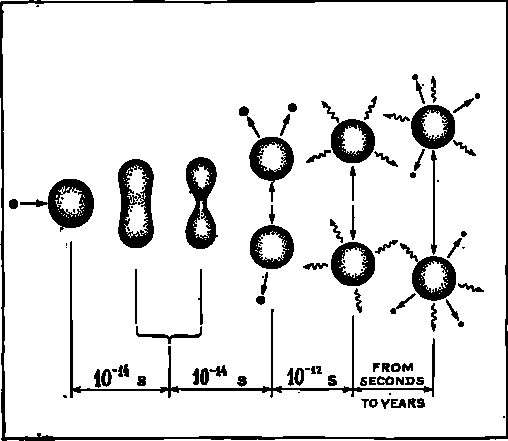
\includegraphics[width=0.9\textwidth]{figures/fig-05-06.pdf}
\caption{The fission of the Uranium-235 nucleus.}
\label{fig-5.6}
\end{figure}

\figr{fig-5.6} is a diagram of one of the most important reactions of this type: the fission of the uranium-235 nucleus. 

The question of the first neutron is simple: it can be found in the atmosphere. If we want a more active ``match'', we can take a tiny mixture of radium and beryl­lium.

A neutron enters the nucleus of a uranium-235: atom which consists of 92 protons and 143 neutrons packed tightly into a sphere of radius of about \SI{d-12}{\centi\meter} and produces an isotope called uranium-236. The visitor de­forms the nucleus and, after a time interval of about \SI{d-14}{\second}, the two halves of the nucleus are held to­gether by a tiny bridge; in another \SI{d-14}{\second} the nu­cleus has split into two pieces. At the same time, each of the fragments ejects two or three (an average of 2.56) neutrons. The fragments fly apart with a colossal kinetic energy. One gram of uranium-235 produces as much energy as 2.5 tons of coal, or \num{22000} kilowatt-hours.

Then, \SI{d-12}{\second} later the nuclei formed in the fission process have more or less calmed down with the emission of eight photons of gamma radiation. The new nuclei are radioactive. Depending on the kind of fragments that have formed, the subsequent process of decay may con­tinue for seconds or for many years with the emission
of gamma rays and the ejection of electrons.

\begin{figure}[!ht]
\centering
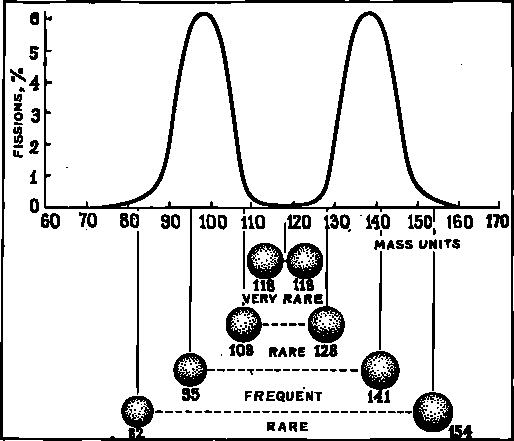
\includegraphics[width=0.9\textwidth]{figures/fig-05-07.pdf}
\caption{The probability of different modes of fission of the Uranium-235 nucleus.}
\label{fig-5.7}
\end{figure}

\figr{fig-5.7} shows that for the most part the nucleus of uranium-235 splits into two unequal fragments. As is evident from a glance at the curve, most fissions result in the formation of nuclei with mass numbers 141 and 95.

The set of newly produced radioactive fragments is very great at any rate. The most varied requirements of industry with respect to artificial radioactive elements can now be satisfied.

If the neutrons formed in the fission of one nucleus can be made to fission the nuclei of other atoms of urani­um, then a chain reaction can be set up.

Since matter is extremely ``full of holes'' as regards its nuclear structure, it is highly probable that the neu­trons formed in the fission of a nucleus will leave the substance without fissioning any other nuclei. What is more, we must not forget that not every encounter between a neutron and a nucleus leads to fission. A chain reaction is ensured only if at each instant of time the number of neutrons located inside a piece of substance is the same or greater than the number at the preceding instant. This condition is stated by the physicist as follows: the neutron multiplication factor -- which is equal to the product of the number of neutrons into the proba­bility of a neutron encountering a nucleus and into the probability of neutron capture by the nucleus -- must not be less than unity.

That is why pure atomic fuel has a critical mass. If this mass is less than critical, one can calmly (well, more or less calmly, let us say) carry a piece of nuclear fuel in one’s pocket. And it won’t be heavy because the critical mass is close to one kilogram.

Naturally, it is very important to know the figure for the critical mass. The first calculations of this quantity were carried out in 1939 by Francis Henri Perrin (1901-1992), the son of Jean Baptiste Perrin (1870-1942). This cal­culation is only of historical interest today because at that time it was not known that a chain reaction cannot develop in natural uranium, no matter how much of it is taken. But not much time was needed for the picture to become quite clear. A chain reaction does not develop in natural uranium because the neutrons produced in the fission of the nuclei of uranium-235 are absorbed via what is called ``resonance'' capture by the atoms of urani­um-238 with the formation of uranium-239, which, by means of two successive beta disintegrations, turns into neptunium and plutonium. Only uranium-235 and plu­tonium possess a critical mass. Substances with a critical mass constitute nuclear fuel. These were the facts that physicists had at their disposal at the beginning of the 1940s.

If a device could be designed in which pressing a button brought together two pieces of nuclear fuel, each of which has a mass less than critical and, when joined, has a mass exceeding the critical mass, then an explosion would take place. That is the simple principle that underlies the working of the atomic bomb.

Now what do we have to do to control the course of a nuclear reaction? Quite obviously we have to create a system containing not only the atoms of the fuel but also other atoms capable of absorbing neutrons and, as it were, putting them out of action. Cadmium rods are quite suitable for this purpose. Cadmium is a good ab­sorber of neutrons. If we make a structure consisting of rods of nuclear fuel and rods of cadmium and then arrange for inserting and extracting the rods (this takes place in the body of a nuclear reactor -- at first it was called a pile), we can set up a nuclear chain reaction by making the neutron multiplication factor slightly more than uni­ty; then we can raise the heat release to the desired level and insert cadmium rods so that the multiplication factor becomes exactly unity.

%\begin{figure}[!ht]
%\centering
%
\includegraphics[width=\textwidth]{figures/fig-03-01.pdf}
%\caption{$X$-rays penetrate muscles and can show the skeleton.}
%\label{fig-3.1}
%\end{figure}

%
%%\newpage
%\begin{center}
%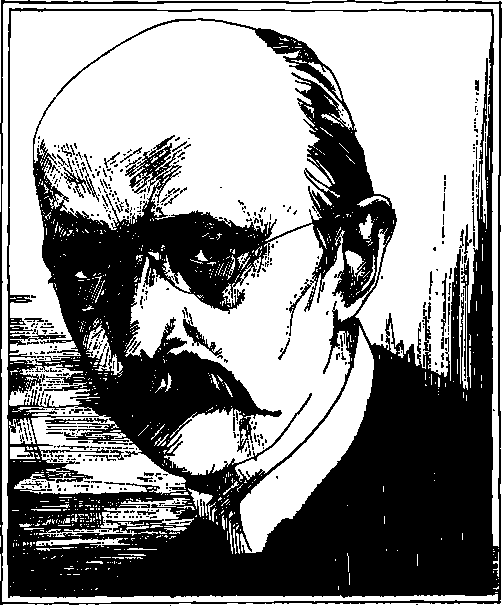
\includegraphics[width=\textwidth]{figures/planck.pdf}
%\end{center}
%{\small \textsf{\hlred{Albert Einstein [1879-1955]}} -- \textsf{\footnotesize the genius who created the theory of relativity and revolutionized all physical thinking. In 1905, Einstein published a treatise devoted to the special theory of relativity. In 1907, he obtained a formula relating energy and the mass of a body. In 1915, Einstein published his general theory of relativity. From this theory there followed new laws of gravita­tion and conclusions concerning the curvature of space.}}



